\documentclass[conference]{IEEEtran}
\IEEEoverridecommandlockouts
% The preceding line is only needed to identify funding in the first footnote. If that is unneeded, please comment it out.
\usepackage{cite}
\usepackage{amsmath,amssymb,amsfonts}
\usepackage{algorithmic}
\usepackage{graphicx}
\usepackage{textcomp}
\usepackage{xcolor}
\usepackage{url}
\usepackage[T1]{fontenc}
\usepackage[utf8]{inputenc}
\def\BibTeX{{\rm B\kern-.05em{\sc i\kern-.025em b}\kern-.08em
    T\kern-.1667em\lower.7ex\hbox{E}\kern-.125emX}}
\begin{document}

\title{Zvučni efekti na gitari\\
%{\footnotesize \textsuperscript{*}Note: Sub-titles are not captured in Xplore and
%should not be used}
%\thanks{Identify applicable funding agency here. If none, delete this.}
}

\author{\IEEEauthorblockN{Magdalena Halusek}
\IEEEauthorblockA{\textit{dept. name of organization (of Aff.)} \\
\textit{name of organization (of Aff.)}\\
City, Country \\
email address}\\
\IEEEauthorblockN{Ivana Šarić}
\IEEEauthorblockA{\textit{dept. name of organization (of Aff.)} \\
\textit{name of organization (of Aff.)}\\
City, Country \\
email address}
\and
\IEEEauthorblockN{Katarina Prgeša}
\IEEEauthorblockA{\textit{dept. name of organization (of Aff.)} \\
\textit{name of organization (of Aff.)}\\
City, Country \\
email address}\\
\IEEEauthorblockN{Ivana Žeger}
\IEEEauthorblockA{\textit{dept. name of organization (of Aff.)} \\
\textit{name of organization (of Aff.)}\\
City, Country \\
email address}
\and
\IEEEauthorblockN{Karla Salamun}
\IEEEauthorblockA{\textit{dept. name of organization (of Aff.)} \\
\textit{name of organization (of Aff.)}\\
City, Country \\
email address}
}

\maketitle

\renewcommand{\figurename}{Slika}

\begin{abstract}
sažetak??
\end{abstract}

\section{Uvod}
Zvuk je mehanički val koji se prenosi određenim medijem. Ljudsko uho je osjetljivo na
frekvencije između otprilike 20 Hz i 20 000 Hz. Jedan je od mnogih oblika kontinuiranih;
analognih signala naše okoline. Ljudski interes za fenomen zvuka traje od najranije povijesti. Do
današnjice je razvijena čitava kultura i tehnologija koja omogućuje stvaranje, snimanje, obradbu
i prijenos zvuka. Pojam povezan sa zvukom koji obuhvaca i ispreplice znanost i umjetnost je glazba.
S ciljem što boljeg doživljaja glazbe, audio signali se obrađuju u kontinuiranoj i
diskretnoj domeni. Mikrofon pretvara zvučne valove u analogni električni sinusni signal. Taj je
signal određen jedinstvenom frekvencijom, brzinom, odstupanjima, itd. Obradba analognim
sklopovima podložna je pogreškama uzrokovanih šumom, preslušavanjem vodova,
temperaturnom ovisnošću, netočnostima nominalnih iznosa elemenata, itd. Da bi se kvalitetno
obradio, kontinuirani signal je potrebno digitalizirati. Digitalna obrada signala se provodi u
računalima. Ima brojne prednosti, poput neosjetljivosti na šum i starenje, laku prilagodbu na
nove zadatke, programabilnost.

Tema projekta je konstruiranje filtara za dodavanje efekata, digitalna obradba snimljenog zvuka
gitare primjenom istih te ispitivanje njihovog utjecaja na signal u vremenskoj i frekvencijskoj
domeni. Razvoj instrumenata i postupaka digitalne obradbe omogućio je eksperimentiranje
zvukom. Glazba se često razvijala upravo iz razloga što su pojedine slučajne greške u sviranju
instrumenata i obradbi snimaka zvuka postale utjecajni zvučni efekti. Zvučni efekti su pojam koji
obuhvaća hardver i softver odgovoran za manipulaciju zvukom. Moguće ih je dodati zvuku u
procesu nastajanja s ciljem da kasnije budu filtrirani ili preoblikovani \cite{b1}, ili
na kraju obrade, u produkcijskoj fazi. Ne postoji jedinstveno pravilo koje je potrebno slijediti pri
odabiru redoslijeda primjene efekata. No, promijenjeni redoslijed uzrokuje promjenu zvuka.
Potrebno je voditi računa o spomenutom obzirom na zvuk koji je poželjno stvoriti. Iako postoje
mnoge vrste i podjele, kao temeljna podjela digitalnih zvučnih efekata
može se navesti sljedeća:

\begin{itemize}
	\item{modulacijski efekti – \textit{Chorus}, \textit{Tremolo}, \textit{Flanger}, \textit{Phaser},}
	\item{vremenski efekti – \textit{Reverb}, kašnjenje, odjek,}
	\item{spektralni efekti – ekvilizacija, \textit{Panning},}
	\item{dinamički efekti – kompresija i distorzija.}
\end{itemize}

Tipični redoslijed efekata za gitaru \cite{b1} jest kompresija – distorzija – ekvilizacija – smanjenje šuma
– modulacija – kašnjenje – odjek.

Filtri po definiciji uklanjaju ili atenuiraju određene frekvencije iz spektra signala iznad
ili ispod neke granične frekvencije. Izjednačivači, pak, pojačavaju ili smanjuju određene frekvencijske
pojaseve, dok druge ne mijenjaju.


\section{Kompresija}

Kompresor djeluje na zvučni signal u cijelosti s ciljem kontrole zvuka i stvaranja \textit{sustain}
efekta. Kompresija je, zapravo, automatska kontrola glasnoće. Zadaća kompresora je smanjenje
dinamičkog raspona signala, tj. varijacije između najglasnijih i najtiših dijelova signala.
Dijelovi signala s velikim amplitudama, odnosno oni glasniji od nekog praga su atenuirani. Oni s
najmanjim amplitudama, tj. tiši od nekog praga su pojačani s namjerom postizanja uravnoteženijeg zvuka
bez distorzije. Kompresijom je omogućeno pojačanje signala bez potrebe za rezanjem (\textit{clippingom}).
Rezultat je dotjeraniji zvuk. Ipak, javlja se potreba za oprezom jer prekomjerna kompresija stvara
zašumljen i bezizražajan zvuk. Gubitak dijela dinamike postaje zamjetan pri slušanju.

Ovim projektom napravljen je kod za usporedbu originalnog i komprimiranog signala u vremenskoj i
frekvencijskoj domeni što je vidljivo na slici \ref{komp_vrijeme}.

\begin{figure}[h]
    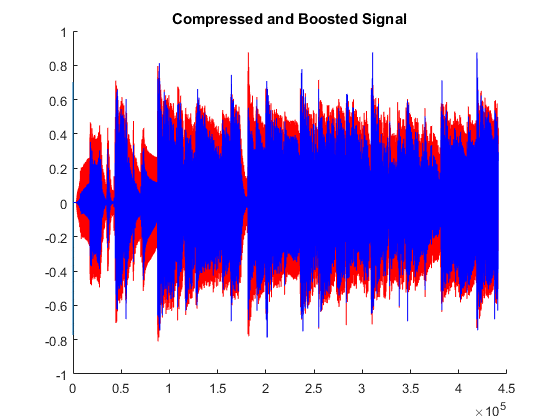
\includegraphics[scale=0.45]{slike/kompresija_vrijeme.png}
    \centering
    \caption{Originalni i komprimirani signal u vremenskoj domeni}							%dodati legend u matlabu
    \label{komp_vrijeme}
\end{figure}

Na slici \ref{komp_spektar} vidljiva je razlika u spektru. Budući da se događaju promjene u amplitudi u
vremenskoj domeni, to je u frekvencijskoj domeni vidljivo kao novonastala istosmjerna komponenta.

\begin{figure}[h]
    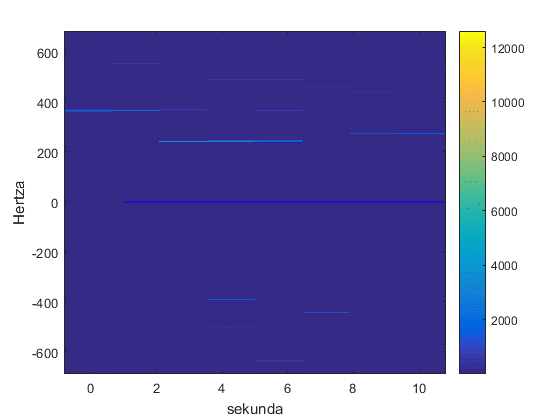
\includegraphics[scale=0.45]{slike/kompresija_spektar.png}
    \centering
    \caption{Spektrogram komprimiranog signala}							%zasto DC komponenta??
    \label{komp_spektar}
\end{figure}

\section{Odjek}

Efekt odjeka temelji se na efektu kašnjenja. Efekt kašnjenja može se opisati kao snimanje ulaznog signala
koji se zatim reproducira nakon određenog vremena. Signal kojemu je dodan efekt kašnjenja, može se
reproducirati više puta ili se ponovno snimiti što stvara ponavljajući zvuk. Osnovna struktura kašnjenja može
se ostvariti pomoću FIR ili IIR filtra ili kombinacijom dvaju filtara. Efekt odjeka može se realizirati pomoću
jednostavnog FIR filtra. Jednadžba FIR filtra kojim se realizira odjek dana je u nastavku.\\
\[y(n) = x(n) + g*x(n-M), M = \tau/f_{s}\]
Gdje:
 \begin{itemize}
   \item{$g$ - predstavlja pojačanje obrađenog signala,}
   \item{$\tau$ - predstavlja iznos kašnjenja signala,}
   \item{$f_{s}$ - predstavlja frekvenciju otipkavanja.}
 \end{itemize}
Dodavanjem efekta odjeka na osnovni signal zvuk poprima dojam odbijanja zvuka od zida, dok se zapravo čuje
ponavljanje osnovnog signala.

Na slici \ref{echo_ulaz} prikazan je spektar ulaznog signala, dok je na slici \ref{echo} prikazan spektar
signala s dodanom jekom. Na spektru obrađenog
signala vide se određene frekvencijske komponente koje se ne mogu vidjeti na spektru ulaznog signala.
Dodatne frekvencijske komponente pojavljuju se upravo zbog ponavljanja signala kroz vrijeme.

\begin{figure}[h]
  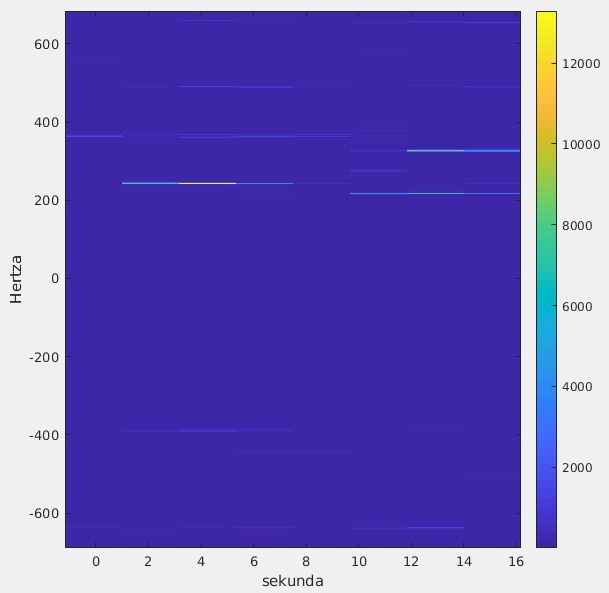
\includegraphics[scale=0.3]{slike/echo_ulaz.jpeg}
  \centering
  \caption{Spektar ualznog signala}
  \label{echo_ulaz}
\end{figure}

\begin{figure}[h]
  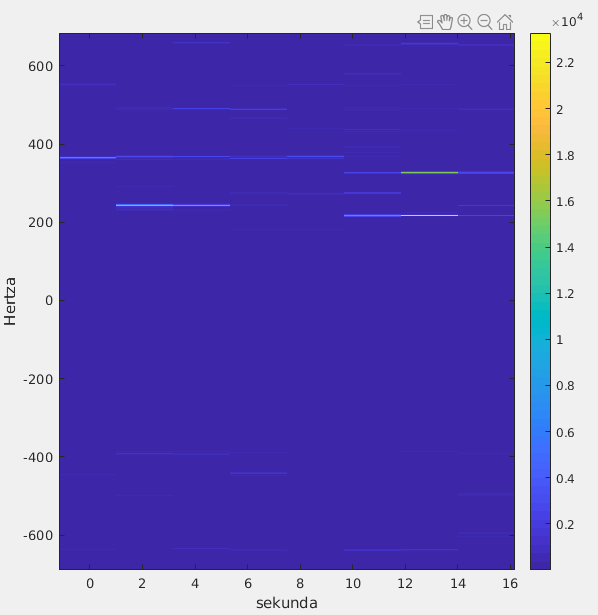
\includegraphics[scale=0.3]{slike/echo.png}
  \centering
  \caption{Spektar obrađenog signala}
  \label{echo}
\end{figure}


\section{Zaključak}
Digitalna obradba signala sastavni je dio glazbene produkcije. Zvučni efekti, često nastali kao
posljedica slučajnih pogrešaka u sviranju i obradbi signala, glavni su faktori u manipulaciji zvukom.

Kompresija smanjuje dinamički raspon signala bez distorzije, bez potrebe za rezanjem
(\textit{clippingom}).

\begin{thebibliography}{00}
\bibitem{b1} Cardiff University, ``Digital Audio Effects'',
	\url{www.cs.cf.ac.uk/Dave/CM0268/PDF/10_CM0268_Audio_FX.pdf}
\end{thebibliography}

\end{document}
